% Standalone Checkly UAT results report.
% The document can also be converted back into an includable section by
% removing the preamble and the \begin{document}/\end{document} pair.
\documentclass[11pt]{article}

\usepackage[a4paper,margin=1in]{geometry}
\usepackage{graphicx}
\usepackage{booktabs}
\usepackage{tabularx}
\usepackage[hidelinks]{hyperref}

\setlength{\parindent}{0pt}
\setlength{\parskip}{0.5em}

\title{Checkly User Acceptance Testing Results}
\author{Checkly}
\date{July 2026}

\begin{document}

\maketitle

\section{User Acceptance Testing Results}
\label{sec:uat-results}

\subsection{Participants and method}

User acceptance testing was conducted with ten participants between 30 June and
10 July 2026. Eight participants were students and two reported a professional
software or office-work background. Six participants tested on a mobile device,
three on a desktop computer, and one on a tablet. Chrome was the most common
browser (six participants). Seven participants had previously used checklist
software occasionally or frequently, while three had never used such software.

Participants rated nine aspects of Checkly on a five-point scale, where higher
scores represented a more favourable evaluation. A rating of 4 or 5 was treated
as positive. Means, medians, sample standard deviations, and response
distributions were examined. Optional open-text responses were coded into
non-exclusive themes. Because the sample was small and convenience-based, the
results are descriptive and should not be generalised to the wider population.

\subsection{Quantitative results}

The quantitative results were generally favourable. Across all nine rating
items, the mean score was 4.12 out of 5 and 73.3\% of the 90 individual ratings
were positive. Overall satisfaction received the highest average score
(\(M=4.4\)), followed by app stability and speed (both \(M=4.3\)). Ease of
checklist creation received the lowest average score (\(M=3.8\)) and the lowest
positive-response rate (60\%).

\begin{table}[htbp]
    \centering
    \small
    \caption{Summary of Checkly UAT ratings (\(N=10\))}
    \label{tab:uat-summary}
    \begin{tabularx}{\textwidth}{Xrrrr}
        \toprule
        Metric & Mean & Median & SD & Positive (\%) \\
        \midrule
        First impression & 4.1 & 5.0 & 1.4 & 70 \\
        Ease of use & 4.0 & 4.5 & 1.3 & 70 \\
        App stability and reliability & 4.3 & 5.0 & 1.3 & 80 \\
        Speed and responsiveness & 4.3 & 5.0 & 1.3 & 80 \\
        Ease of checklist creation & 3.8 & 4.5 & 1.5 & 60 \\
        Usefulness of AI features & 4.0 & 5.0 & 1.5 & 70 \\
        AI understanding of requests & 4.1 & 5.0 & 1.4 & 70 \\
        Trust in AI suggested changes & 4.1 & 4.0 & 1.0 & 80 \\
        Overall satisfaction & 4.4 & 5.0 & 1.1 & 80 \\
        \bottomrule
    \end{tabularx}
\end{table}

Figure~\ref{fig:uat-means} compares the mean score for each metric. The orange
bar highlights checklist creation, the only metric with a mean below 4.0.

\begin{figure}[htbp]
    \centering
    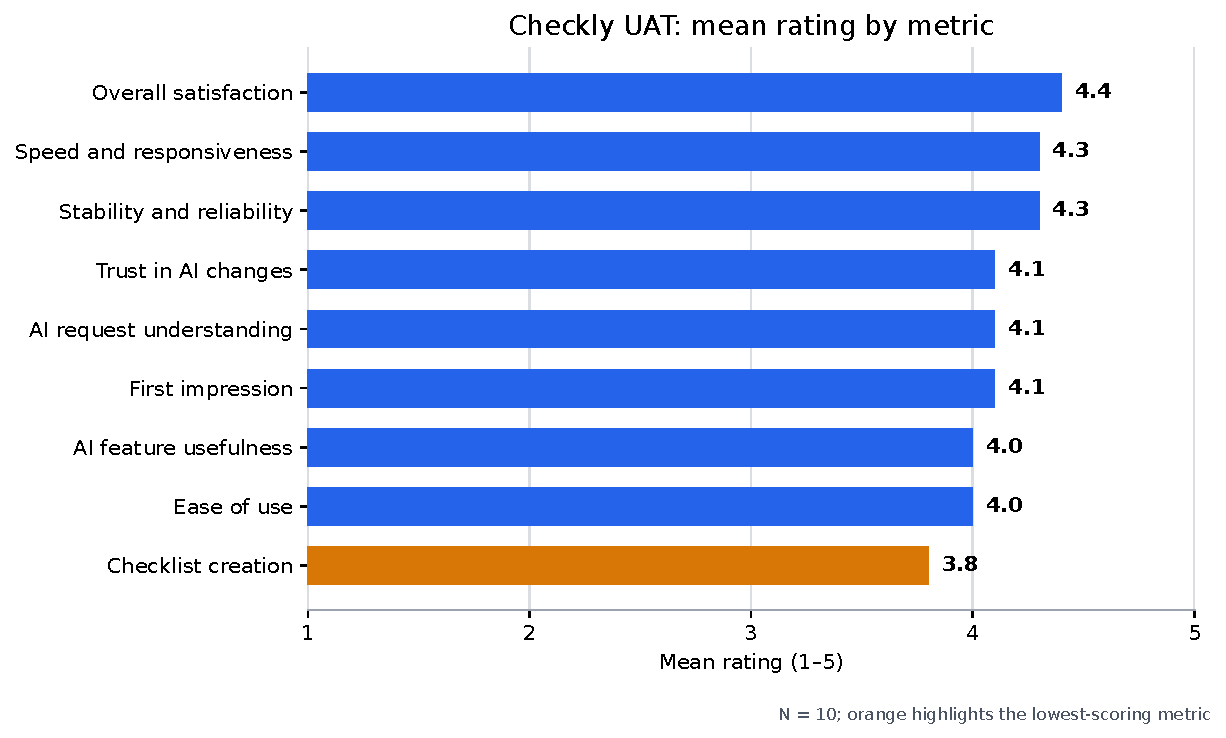
\includegraphics[width=0.95\textwidth]{figures/uat_metric_averages.pdf}
    \caption{Mean rating for each UAT metric on the five-point scale.}
    \label{fig:uat-means}
\end{figure}

Figure~\ref{fig:uat-distribution} shows the complete rating distribution. This
is important for the small sample because one participant gave consistently low
scores across most items. The response was retained, and the medians and full
distributions are reported so that its influence on the means remains visible.

\begin{figure}[htbp]
    \centering
    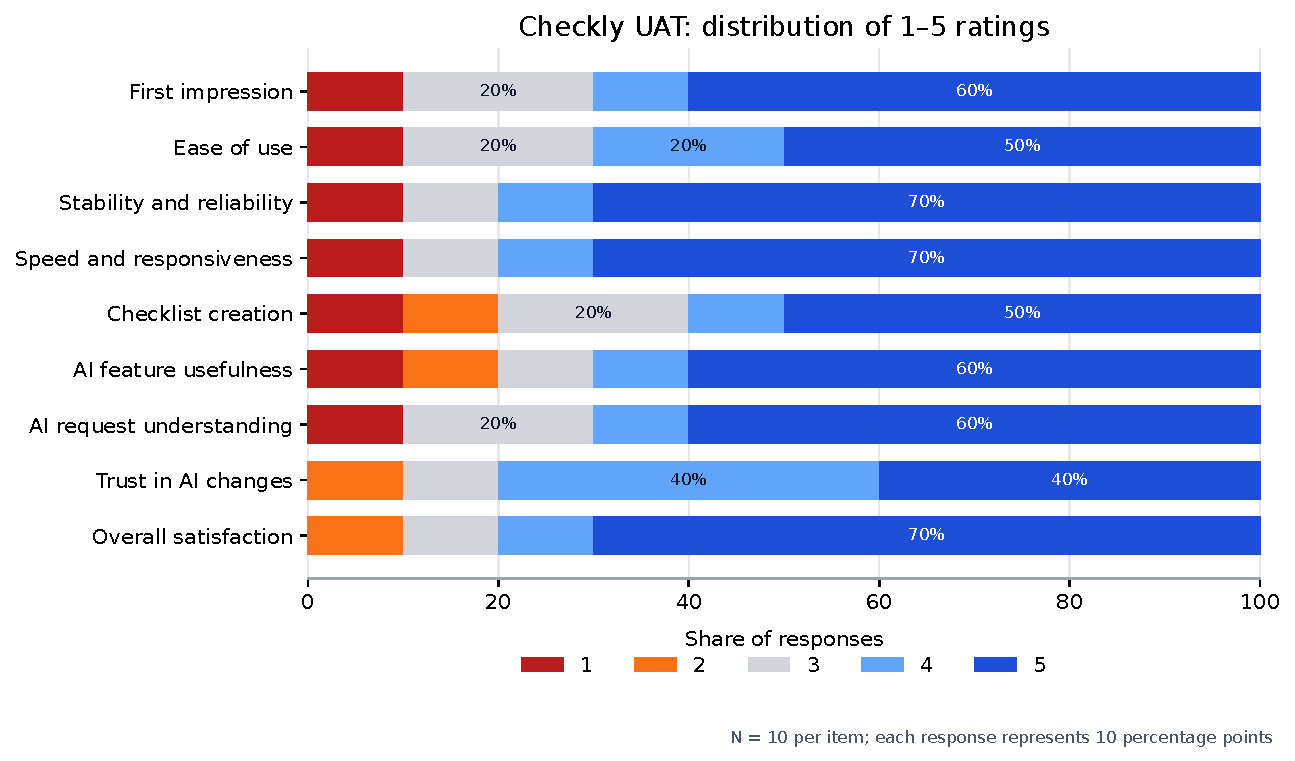
\includegraphics[width=0.98\textwidth]{figures/uat_likert_distribution.pdf}
    \caption{Distribution of the 1--5 ratings for each UAT metric.}
    \label{fig:uat-distribution}
\end{figure}

All ten participants answered ``Yes'' when asked whether there was any chance
that they would use Checkly in the future. This indicates universal future-use
interest within the test sample, although the wording measures possibility
rather than definite adoption intent.

\subsection{Qualitative feedback}

The AI capabilities were the most frequently praised theme, mentioned by four
participants. Participants particularly valued the assistant's ability to
understand natural-language requests and modify checklists directly. UI and
visual design were praised by three participants, while simplicity and checklist
organisation received additional positive mentions.

The most repeated improvement themes were the PDF/download workflow and layout
simplification, each mentioned by three participants. Two participants raised
sign-up or onboarding concerns. Individual suggestions included direct access
to checklists, clearer navigation, item check-off controls, legal information,
social proof, and profile customisation. Figure~\ref{fig:uat-themes} summarises
the coded improvement themes. Since comments were optional and themes were
non-exclusive, the counts should not be interpreted as population percentages.

\begin{figure}[htbp]
    \centering
    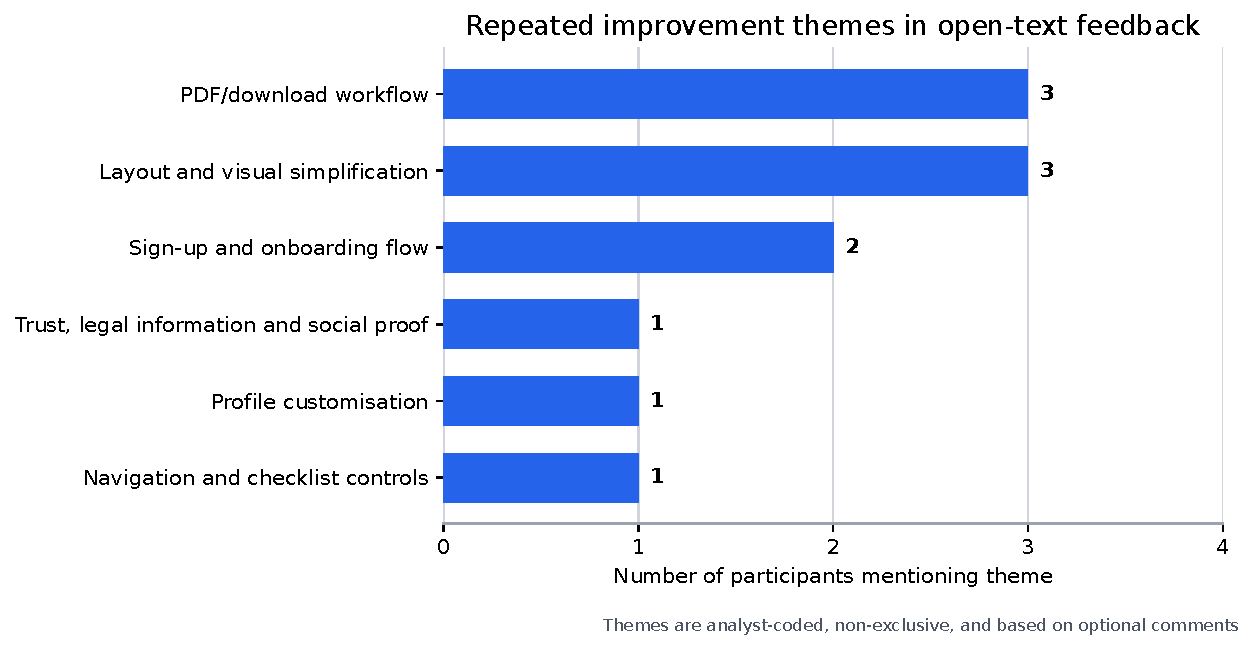
\includegraphics[width=0.95\textwidth]{figures/uat_improvement_themes.pdf}
    \caption{Improvement themes identified in the optional open-text feedback.}
    \label{fig:uat-themes}
\end{figure}

\subsection{Acceptance assessment and recommendations}

No predefined acceptance threshold or critical-defect log was supplied.
Consequently, the survey evidence alone cannot establish a formal pass or fail.
The results support a \emph{conditionally favourable} assessment: overall
satisfaction, performance, reliability, and future-use interest were strong,
but the checklist-creation and PDF workflow requires further attention. For
illustration, if acceptance required a mean of at least 4.0 and at least 70\%
positive responses, every metric except checklist creation would meet the rule.

The recommended actions are:

\begin{enumerate}
    \item Correct and simplify the PDF upload, creation, and download workflow,
          then repeat the associated task on mobile devices.
    \item Simplify the responsive layout, reduce visual density, and ensure the
          primary checklist view fits comfortably within the viewport.
    \item Allow users to create a checklist before requiring registration, or
          make the sign-up point and its purpose clearer.
    \item Review checklist navigation and controls, including direct checklist
          access, item check-off behaviour, and back navigation.
    \item Follow up with the consistently low-scoring participant, if possible,
          because no open-text explanation was provided for those scores.
\end{enumerate}

A final acceptance decision should combine these survey findings with the
severity and resolution status of observed defects and the outcome of regression
testing after the priority changes are implemented.

\end{document}
